\documentclass[ignorenonframetext, hyperref=unicode]{beamer}



\usepackage{cmap}
%\usepackage[T2A]{fontenc}
\usepackage[utf8]{inputenc}
\usepackage[bulgarian]{babel}
\selectlanguage{bulgarian}

\usepackage{color}
\usepackage{graphicx}
\usepackage{listings}
\usepackage{rcsinfo}
\usepackage{pgf}
\usepackage{supertabular}
\usepackage{rotating}

\hypersetup{
	colorlinks=true,
	linkcolor=blue,
	filecolor=blue,
	urlcolor=blue,
	anchorcolor=blue,
	citecolor=blue
}

\lstset{language=C++, 
  numbers=left, 
  numberstyle=\tiny,
  stepnumber=1, 
  numbersep=3pt, 
  tabsize=2, 
  texcl,
  basicstyle=\ttfamily\small,
  identifierstyle=\ttfamily\small,
  keywordstyle=\sffamily\bfseries\small,
  extendedchars=true, inputencoding=utf8,
  backgroundcolor=\color[rgb]{1,1,0.845},
  escapeinside={/*@}{@*/}}

%\usepackage{algpseudocode}
%\usepackage[ruled]{algorithm}

\newcommand{\Cpp}{{\ttfamily\bfseries C++}}
\newcommand{\CC}{{\ttfamily\bfseries C}}

\definecolor{outputcolor}{rgb}{0.0,0.0,0.5}
\newcommand{\aout}[1]{\color{outputcolor}{\begin{verbatim}#1\end{verbatim}}}

% \usepackage[T2A]{fontenc}
% \usepackage[cp1251]{inputenc}
% \usepackage[bulgarian]{babel}
\selectlanguage{bulgarian}




\newcommand{\lubo}{%
\author[Л.~Чорбаджиев]{Любомир Чорбаджиев\inst{1} \\ 
{\ttfamily lchorbadjiev@elsys-bg.org}}
\institute[ELSYS] % (optional, but mostly needed)
{
\inst{1}%
Технологическо училище ``Електронни системи'' \\
Технически университет, София
}}

\newcommand{\osauthors}{%
\author{
	В.Кетипов\\ 
	\and
	Н.Димитров \\ 
	\and
	{Х.Стефанов \\
	{\ttfamily elsys.os.2014@gmail.com}}
}
\institute[ELSYS] % (optional, but mostly needed)
{
\inst{1}%
Технологическо училище ``Електронни системи'' \\
Технически университет, София
}}

\titlegraphic{\href{http://creativecommons.org/licenses/by-sa/3.0/}{\includegraphics{../macros/cc.png}}}

\newcommand{\ie}{т.~е.\ }

\newcounter{probcounter}[section]
\newenvironment{prob}[1][]%
        {\smallskip%
         \noindent\refstepcounter{probcounter}%
          \textbf{\theprobcounter${}^{#1}$.}\ }%
   {\medskip}

\mode<article>
{

}

\mode<presentation>
{
  \usetheme[secheader=true]{Madrid}
  \usecolortheme{crane}
  \usefonttheme[onlylarge]{structurebold}
  \setbeamercovered{transparent}
}

\usepackage[unicode]{hyperref}

%%% Local Variables: 
%%% mode: latex
%%% TeX-master: t
%%% End: 


\title[Памет {(\em\rcsInfoRevision)}]{Управление на паметта} 
\lubo
\date{\today}

\begin{document}

\frame{\maketitle}

\begin{frame}
\frametitle{Съдържание}
\tableofcontents %[hideallsubsections]
\end{frame}

%-------------------------------------------------------------------- SECTION -
\section{Въведение}

%---------------------------------------------------------------------- SLIDE -
\begin{frame}
\frametitle{Въведение}
\begin{itemize}
  \item За да бъде изпълнена една програма, първо тя трябва да бъде заредена в
  оперативната памет на компютърната система.
  \item {\em Входна опашка} се нарича опашка от процеси, които чакат да бъдат
  заредени в оперативната памет на компютъра, за да бъдат изпълнени.
  \item Потребителската програма преминава през няколко стъпки преди да бъде
  изпълнена.
\end{itemize}
\end{frame}

%---------------------------------------------------------------------- SLIDE -
\begin{frame}
\frametitle{Въведение}
\begin{figure}[h]
\center
\scalebox{0.315}{\includegraphics{pics/silberschatz7e-8-7}}
\caption{Silberschatz, Gavin, Gagne: {\em Operating Systems Concepts}}
\end{figure}
\end{frame}

%---------------------------------------------------------------------- SLIDE -
\begin{frame}
\frametitle{Базов и граничен регистър}
\begin{figure}[h]
\center
\scalebox{0.5}{\includegraphics{pics/02-memory-protection}}
\end{figure}
\end{frame}

%---------------------------------------------------------------------- SLIDE -
\begin{frame}
\frametitle{Базов и граничен регистър}
\begin{figure}[h]
\center
\scalebox{0.5}{\includegraphics{pics/02-memory-protection-algo}}
\end{figure}
\end{frame}

\section{Основни концепции}
%---------------------------------------------------------------------- SLIDE -
\begin{frame}
\frametitle{Свързване на програмата с адреси в паметта}
Свързването на инструкциите и данните на програмата с адреси в оперативната
памет на компютъра може да се реализира в различни моменти от жизнения цикъл на
програмата.
\begin{itemize}
  \item {\em По време на компилация:} Ако разположението на програмата в
  паметта е известно предварително, още по време на компилация на програмата,
  то компилатора може да генерира абсолютни адреси в паметта. Ако трябва да се
  промени разположението в паметта на програмата, то е необходима тя да се
  прекомпилира.
\end{itemize}
\end{frame}

%---------------------------------------------------------------------- SLIDE -
\begin{frame}
\frametitle{Свързване на програмата с адреси в паметта}
\begin{itemize}
  \item {\em По време на зареждане:} Когато разположението на програмата в
  паметта не е предварително известно, то е необходимо компилаторът да генерира
  {\em преместваем} код.
  \item {\em По време на изпълнение:} Свързването на програмата с адреси в
  оперативната памет може да се отложи до момента на изпълнение на програмата,
  ако програмата (или части от нея) могат да бъдат преместени от един сегмент на
  оперативната памет в друг. За тази цел обикновено е необходима хардуерна
  поддръжка.
\end{itemize}
\end{frame}

%---------------------------------------------------------------------- SLIDE -
\begin{frame}
\frametitle{Логически и физически адреси}
\begin{itemize}
  \item Логически адрес се нарича адрес, генериран от централния процесор.
  Понякога тези адреси се наричат виртуални адреси.
  \item Физически адрес е адресът на клетката от оперативната памет, който се
  зарежда върху шината за адресиране.
  \item Разделянето на концепциите за логическо и физическо адресно
  пространство има основно значение за управлението на паметта.
  \item Управлението на паметта се заключава в начините, по които логическото
  адресно пространство се свързва с физическото адресно пространство.
\end{itemize}
\end{frame}

%---------------------------------------------------------------------- SLIDE -
\begin{frame}
\frametitle{Логически и физически адреси}
\begin{itemize}
  \item В случаите на свързване на адреси при компилация и по време на
  зареждане на програмата, логическите и физическите адреси съвпадат.
  \item При използване на подхода за свързване на адресите по време на
  изпълнение, логическите и физическите адреси са различни.
\end{itemize}
\end{frame}

%---------------------------------------------------------------------- SLIDE -
\begin{frame}
\frametitle{Блок за управление на паметта (MMU)}
\begin{itemize}
  \item Блок за управление на паметта се нарича част от хардуера (централния
  процесор), който се използва за изграждане на съответствие между 
  логическите и физическите адреси.
  \item Основен елемент на блока за управление на паметта е регистърът за
  преместване (базов регистър) (relocation register, base register), който се
  добавя към всеки генериран от централния процесор логически адрес в момента,
  в който централния процесор се обръща към паметта.
  \item Потребителската програма работи само с логически адреси — тя никога не
  използва физически адреси.
\end{itemize}
\end{frame}

%---------------------------------------------------------------------- SLIDE -
\begin{frame}
\frametitle{Блок за управление на паметта (MMU)}
\begin{figure}[h]
\center
\scalebox{0.315}{\includegraphics{pics/silberschatz7e-8-10}}
\caption{Silberschatz, Gavin, Gagne: {\em Operating Systems Concepts}}
\end{figure}
\end{frame}

\section{Динамично зареждане и свързване}

%---------------------------------------------------------------------- SLIDE -
\begin{frame}
\frametitle{Динамично зареждане}
\begin{itemize}
  \item Зареждането в паметта на функциите и подпрограмите се отлага до
  момента, в който те действително са необходими (мързеливо зареждане).
  \item Този подход позволява по-добро използване на паметта -- функциите и
  подпрограмите които не се използват, не се зареждат в оперативната памет.
  Когато големи участъци от кода са предназначени за обработка на рядко
  случващи се ситуации, динамичното зареждане води до значително по-добро
  използване на паметта.
  \item Динамичното зареждане не изисква специална поддръжка от операционната
  система. То може да бъде реализирано изцяло в потребителската програма.
\end{itemize}
\end{frame}

%---------------------------------------------------------------------- SLIDE -
\begin{frame}
\frametitle{Динамично свързване}
\begin{itemize}
  \item Динамичното свързване е особено полезно при реализиране на библиотеки.
  \item В кода на приложението се интегрират малки участъци код, наречени {\em
  стъбове (stub)}, чиято задача е да намерят правилната, заредена вече в
  оперативната памет функция.
  \item Когато стъбът намери необходимата функция, той се заменя с адреса на
  тази функция и я извиква.
  \item Операционната система трябва да провери дали съответната функция е в
  адресното пространство на процеса, който я извиква.
\end{itemize}
\end{frame}

%---------------------------------------------------------------------- SLIDE -
\begin{frame}
\frametitle{Препокриване (Overlay)}
\begin{figure}[h]
\center
\scalebox{0.3}{\includegraphics{pics/silberschatz6e-9-11}}
\caption{Silberschatz, Gavin, Gagne: {\em Operating Systems Concepts}}
\end{figure}
\end{frame}


\section{Размяна (swapping)}

% %---------------------------------------------------------------------- SLIDE -
% \begin{frame}
% \frametitle{Размяна (swapping)}
% \begin{itemize}
%   \item 
% \end{itemize}
% \end{frame}

%---------------------------------------------------------------------- SLIDE -
\begin{frame}
\frametitle{Размяна (swapping)}
\begin{figure}[h]
\center
\scalebox{0.25}{\includegraphics{pics/silberschatz6e-9-13}}
\caption{Silberschatz, Gavin, Gagne: {\em Operating Systems Concepts}}
\end{figure}
\end{frame}

\section{Раздели в оперативната памет}
%---------------------------------------------------------------------- SLIDE -
\begin{frame}
\frametitle{Фиксирани раздели}
\begin{itemize}
  \item Оперативната памет се разделя на определен брой и с определен размер
  парчета -- раздели.
  \item В първите операционни системи често се използва във варианта два
  фиксирани раздела -- един за резидентния монитор (операционна система) и
  втори раздел за потребителското задание.
  \item Този подход може да се комбинира със свързването на физическите адреси
  по време на компилация. По време на компилация се определя в кой точно раздел
  ще работи дадена програма и компилаторът и свързващият редактор генерират
  абсолютни адреси.
  \item По-гъвкаво е да се използва преместваем обектен код -- свързването на
  физическите адреси да става по време на зареждане на програмата, в зависимост
  от това в кой раздел се зарежда тя.
\end{itemize}
\end{frame}

%---------------------------------------------------------------------- SLIDE -
\begin{frame}
\frametitle{Фиксирани раздели}
\begin{figure}[h]
\center
\scalebox{0.35}{\includegraphics{pics/silberschatz6e-9-15}}
\caption{Silberschatz, Gavin, Gagne: {\em Operating Systems Concepts}}
\end{figure}
\end{frame}

%---------------------------------------------------------------------- SLIDE -
\begin{frame}
\frametitle{Фрагментация}
\begin{itemize}
  \item Наличието на неизползвани участъци от паметта се нарича {\em
  фрагментация}
  \item Една от основните причини за фрагментация на оперативната памет при
  фиксираните раздели е, че част от раздела не се използва, тъй като размерът на
  раздела е фиксирана и не може да се променя.
\end{itemize}
\end{frame}

%---------------------------------------------------------------------- SLIDE -
\begin{frame}
\frametitle{Фрагментация}
\begin{itemize}
  \item Фрагментацията на оперативната памет се разделя на два вида:
  \begin{itemize}
    \item {\em Външна фрагментация} -- съществува свободна оперативна памет, но
    тя е разделена на малки дупки между разделите, които се използват от работещите
    процеси.
    \item {\em Вътрешна фрагментация} -- заделената памет е по-голяма от
    паметта, която реално се използва от процеса; тази памет е вътрешна за раздела, но
    не се използва от процеса.
  \end{itemize}
  
\end{itemize}
\end{frame}

%---------------------------------------------------------------------- SLIDE -
\begin{frame}
\frametitle{Променливи раздели}
\begin{itemize}
  \item {\em Дупка} -- свободен участък от оперативната памет. 
  \item Първоначално цялата оперативна памет (преди да се заредят процеси)
  може да се разглежда като една ``дупка''.
  \item Когато един процес трябва да бъде зареден в оперативната памет, то за
  него се заделя памет от някоя от дупките, които са достатъчно големи за да
  поберат процеса.
  \item Операционната система трябва да съхранява информацията за заетите
  раздели и за свободните раздели (дупки) в оперативната памет.
  \item Този подход също страда от фрагментация. 
\end{itemize}
\end{frame}


%---------------------------------------------------------------------- SLIDE -
\begin{frame}
\frametitle{Уплътняване}
\begin{itemize}
  \item Възможен подход за справяне с фрагментацията при променливите раздели е
  {\em уплътняването} на оперативната памет.
  \item Идеята е всички процеси да се преместят в оперативната памет така, че
  да остане само една дупка.
  \item Този подход има ред недостатъци:
  \begin{itemize}
    \item Местенето на процеси обаче, е времеемко. 
    \item Докато се местят процесите
  трябва да бъдат спрени.
  \end{itemize}
  \item Поради тези недостатъци уплътняването на оперативната памет се използва
  рядко.
\end{itemize}
\end{frame}

%---------------------------------------------------------------------- SLIDE -
\begin{frame}
\frametitle{Стратегии за избиране на раздел}
Нека си представим, че са стартира нов процес, който има нужда от $N$
байта оперативна памет. Възможните стратегии за избор на подходящ раздел от
паметта се следните:
\begin{itemize}
  \item {\em Първият подходящ:} избира се първата дупка в паметта, която е
  достатъчно голяма.
  \item {\em Най-подходящият:} избира се най-малката дупка в паметта, която е
  достатъчно голяма. 
  \item {\em Най-неподходящият:} избира се най-голямата дупка в оперативната
  памет.
\end{itemize}
Моделиране на тези стратегии показва, че стратегиите ``първият подходящ'' и
``най-подходящият'' имат по-добра производителност от гледна точка на
бързодействие и използваемост на оперативната памет. Това са най-често
използваните стратегии при работа с раздели.
\end{frame}


\section{Делене на страници}
%---------------------------------------------------------------------- SLIDE -
\begin{frame}
\frametitle{Делене на страници}
\begin{itemize}
  \item Логическото и физическото адресно пространство на процеса не са
  непрекъснати (един раздел), а са разделени на парчета.
  \item Физическото адресно пространство е разделено на фиксирани по размер
  блоково, които се наричат {\em кадри (frames)}. Типично като размер на кадъра
  се избира число, степен на 2 -- да речем 512, 1024,\ldots
  \item Логическото адресно пространство се разделя на блокове със същия размер
  (като размера на кадъра), които се наричат {\em страници (pages)}.
  \item Операционната система трябва да съхранява информация за всички свободни
  кадри.
\end{itemize}
\end{frame}

%---------------------------------------------------------------------- SLIDE -
\begin{frame}
\frametitle{Делене на страници}
\begin{itemize}
  \item За да се зареди една програма с размер $N$ страници в оперативната
  памет е необходимо операционната система да намери съответния брой свободни
  кадри, да зареди програмата и да инициализира таблицата за преобразуване на
  логическите във физически адреси.
  \item Деленето на страници води до увеличаване на вътрешната фрагментация.
\end{itemize}
\end{frame}

%---------------------------------------------------------------------- SLIDE -
\begin{frame}
\frametitle{Преобразуване на адреси}
\begin{itemize}
  \item Всеки логически адрес генериран от централния процесор се разделя на
  две: {\em номер на страница (p)} и {\em отместване в страницата (d)}.
  \item Номерът на страницата (p) се използва като индекс в {\em
  преобразуващата таблица (таблицата на страниците, page table)}, където се
  съхранява базовия адрес на кадъра, съответстващ на дадената страница.
  \item Отместването в страницата (d) се добавя към базовия адрес на кадъра за
  да се получи физическия в оперативната памет.
\end{itemize}
\end{frame}

%---------------------------------------------------------------------- SLIDE -
\begin{frame}
\frametitle{Преобразуване на адреси}
\begin{figure}[h]
\center
\scalebox{0.29}{\includegraphics{pics/silberschatz6e-9-21}}
\caption{Silberschatz, Gavin, Gagne: {\em Operating Systems Concepts}}
\end{figure}
\end{frame}

%---------------------------------------------------------------------- SLIDE -
\begin{frame}
\frametitle{Страници}
\begin{figure}[h]
\center
\scalebox{0.23}{\includegraphics{pics/silberschatz6e-9-22}}
\caption{Silberschatz, Gavin, Gagne: {\em Operating Systems Concepts}}
\end{figure}
\end{frame}

%---------------------------------------------------------------------- SLIDE -
\begin{frame}
\frametitle{Страници}
\begin{figure}[h]
\center
\scalebox{0.28}{\includegraphics{pics/silberschatz6e-9-23}}
\caption{Silberschatz, Gavin, Gagne: {\em Operating Systems Concepts}}
\end{figure}
\end{frame}

%---------------------------------------------------------------------- SLIDE -
\begin{frame}
\frametitle{Свободни кадри}
\begin{figure}[h]
\center
\scalebox{0.31}{\includegraphics{pics/silberschatz6e-9-24}}
\caption{Silberschatz, Gavin, Gagne: {\em Operating Systems Concepts}}
\end{figure}
\end{frame}

%---------------------------------------------------------------------- SLIDE -
\begin{frame}
\frametitle{Преобразуваща таблица}
\begin{itemize}
  \item Преобразуващата таблица (page table) типично се съхранява в оперативната
  памет.
  \item При такъв подход достъпът до данните и инструкциите изисква две
  обръщания към паметта -- веднъж към преобразуващата таблица за да се формира
  физическия адрес и веднъж към съответния адрес в оперативната памет.
  \item Този проблем може да бъде решен като се използва специализиран бърз
  хардуерен кеш, който е организиран като асоциативна памет (associative
  memory, translation look-aside buffer (TLB)).
\end{itemize}
\end{frame}

%---------------------------------------------------------------------- SLIDE -
\begin{frame}
\frametitle{Преобразуваща таблица}
\begin{figure}[h]
\center
\scalebox{0.285}{\includegraphics{pics/silberschatz6e-9-27}}
\caption{Silberschatz, Gavin, Gagne: {\em Operating Systems Concepts}}
\end{figure}
\end{frame}


%---------------------------------------------------------------------- SLIDE -
\begin{frame}
\frametitle{Защита на паметта}
\begin{itemize}
  \item Защитата на паметта при деленето на страници се реализира като с всеки
  кадър се асоциира допълнителен бит (или битове).
  \item Най-простата схема асоциира с всяка страница в таблицата за
  преобразуване допълнителен бит за валидност на страницата (valid/invalid bit).
  \item Когато битът е в състояние ``валиден (valid)'', то това означава че
  страницата е в логическото адресно пространство на процеса и следователно
  може да бъде използвана (адресирана).
  \item Когато битът е в състояние ``невалиден (invalid)'', то това означава,
  че страницата не е в логическото адресно пространство.
\end{itemize}
\end{frame}

%---------------------------------------------------------------------- SLIDE -
\begin{frame}
\frametitle{Преобразуваща таблица}
\begin{figure}[h]
\center
\scalebox{0.285}{\includegraphics{pics/silberschatz6e-9-30}}
\caption{Silberschatz, Gavin, Gagne: {\em Operating Systems Concepts}}
\end{figure}
\end{frame}

%---------------------------------------------------------------------- SLIDE -
\begin{frame}
\frametitle{Видове преобразуващи таблици}
\begin{itemize}
  \item Йерархични преобразуващи таблици.
  \item Преобразуващи хеш-таблици.
  \item Обърнати преобразуващи таблици.
\end{itemize}
\end{frame}


%---------------------------------------------------------------------- SLIDE -
\begin{frame}
\frametitle{Йерархична преобразуваща таблица с две нива}
\begin{figure}[h]
\center
\scalebox{0.23}{\includegraphics{pics/silberschatz6e-9-34}}
\caption{Silberschatz, Gavin, Gagne: {\em Operating Systems Concepts}}
\end{figure}
\end{frame}


%---------------------------------------------------------------------- SLIDE -
\begin{frame}
\frametitle{Йерархична преобразуваща таблица с две нива}
\begin{figure}[h]
\center
\scalebox{0.32}{\includegraphics{pics/silberschatz6e-9-35}}
\caption{Silberschatz, Gavin, Gagne: {\em Operating Systems Concepts}}
\end{figure}
\end{frame}

%---------------------------------------------------------------------- SLIDE -
\begin{frame}
\frametitle{Преобразуваща хеш-таблица}
\begin{figure}[h]
\center
\scalebox{0.35}{\includegraphics{pics/silberschatz6e-9-37}}
\caption{Silberschatz, Gavin, Gagne: {\em Operating Systems Concepts}}
\end{figure}
\end{frame}

%---------------------------------------------------------------------- SLIDE -
\begin{frame}
\frametitle{Общи страници}
\begin{figure}[h]
\center
\scalebox{0.24}{\includegraphics{pics/silberschatz6e-9-41}}
\caption{Silberschatz, Gavin, Gagne: {\em Operating Systems Concepts}}
\end{figure}
\end{frame}

\section{Сегментна организация}
%---------------------------------------------------------------------- SLIDE -
\begin{frame}
\frametitle{Сегментна организация}
\begin{itemize}
  \item Сегментната организация на оперативната памет позволява програмата да
  бъде разположена в няколко несъседни участъка от паметта.
  \item Сегментната организация е схема за управление на паметта, която
  поддържа гледната точка на потребителя върху организацията на оперативната
  памет. 
  \item Програмата е разделена на съвкупност от сегменти. Всеки сегмент е
  логическа част от програмата -- например функция, метод, обект, локални
  променливи, глобални променливи, масив и т.н.
  \item Това, че програмата може да бъде разделена на сегменти, позволява да се
  намали външната фрагментация.
\end{itemize}
\end{frame}

%---------------------------------------------------------------------- SLIDE -
\begin{frame}
\frametitle{Сегментна организация}
\begin{figure}[h]
\center
\scalebox{0.29}{\includegraphics{pics/silberschatz6e-9-43}}
\caption{Silberschatz, Gavin, Gagne: {\em Operating Systems Concepts}}
\end{figure}
\end{frame}

%---------------------------------------------------------------------- SLIDE -
\begin{frame}
\frametitle{Сегментна организация}
\begin{figure}[h]
\center
\scalebox{0.45}{\includegraphics{pics/silberschatz6e-9-44}}
\caption{Silberschatz, Gavin, Gagne: {\em Operating Systems Concepts}}
\end{figure}
\end{frame}

%---------------------------------------------------------------------- SLIDE -
\begin{frame}
\frametitle{Сегментна организация}
\begin{itemize}
  \item Логическият адрес при сегментната организация се състои от двойката
  $<s,d>$, където $s$ е номер на сегмент, а $d$ е отместване в рамките на
  сегмента.
  \item За изобразяване на логическите адреси във физически се използва
  {\em таблица на сегментите}.
  \item Всеки елемент на таблицата на сегментите съдържа {\em базов адрес} и
  {\em граница}. Базовият адрес е началния адрес във физическата памет, от
  който е разположен сегмента. Границата съдържа размера на сегмента.
\end{itemize}
\end{frame}

%---------------------------------------------------------------------- SLIDE -
\begin{frame}
\frametitle{Сегментна организация}
\begin{itemize}
  \item Таблицата на сегментите е разположена в оперативната памет. 
  \item Регистърът за начален адрес на таблицата на сегментите (segment-table
  base register - STBR) сочи към началото на таблицата на сегментите.
  \item Регистърът за размера на таблицата на сегментите (segment-table
  length register - STLR) съдържа броя на сегментите, които се използват от
  процеса. Номерът на сегмент, генериран от процесора е валиден, ако е по-малък
  от STLR.
\end{itemize}
\end{frame}

%---------------------------------------------------------------------- SLIDE -
\begin{frame}
\frametitle{Сегментна организация: защита на паметта}
\begin{itemize}
  \item Сегментите отразяват логическите части на програмата -- код на
  програмата, програмен стек, данни и т.н.
  \item Към всеки елемент от таблицата на сегментите е асоцииран набор от
  допълнителни битове, предназначени за контрол на достъпа до съответния
  сегмент.
  \item С всеки сегмент се свързват определени права за достъп -- права за
  четене, права за писане и права за изпълнение.
  \item Например: на сегмент, който съдържа изпълнимия код на програмата, се
  назначават права само за изпълнение. Четенето и писането в този
  сегмент се забраняват.
\end{itemize}
\end{frame}

%---------------------------------------------------------------------- SLIDE -
\begin{frame}
\frametitle{Сегментна организация}
\begin{figure}[h]
\center
\scalebox{0.3}{\includegraphics{pics/silberschatz6e-9-48}}
\caption{Silberschatz, Gavin, Gagne: {\em Operating Systems Concepts}}
\end{figure}
\end{frame}

%---------------------------------------------------------------------- SLIDE -
\begin{frame}
\frametitle{Сегментна организация}
\begin{figure}[h]
\center
\scalebox{0.28}{\includegraphics{pics/silberschatz6e-9-49}}
\caption{Silberschatz, Gavin, Gagne: {\em Operating Systems Concepts}}
\end{figure}
\end{frame}

%---------------------------------------------------------------------- SLIDE -
\begin{frame}
\frametitle{Сегментна организация: общи сегменти}
\begin{figure}[h]
\center
\scalebox{0.24}{\includegraphics{pics/silberschatz6e-9-50}}
\caption{Silberschatz, Gavin, Gagne: {\em Operating Systems Concepts}}
\end{figure}
\end{frame}

%---------------------------------------------------------------------- SLIDE -
\begin{frame}
\frametitle{Смесена организация: странично-сегментна}
\begin{figure}[h]
\center
\scalebox{0.24}{\includegraphics{pics/silberschatz6e-9-52}}
\caption{Silberschatz, Gavin, Gagne: {\em Operating Systems Concepts}}
\end{figure}
\end{frame}



\section{Виртуална памет}
%---------------------------------------------------------------------- SLIDE -
\begin{frame}
\frametitle{Виртуална памет}
\begin{itemize}
  \item {\em Виртуална памет} се нарича концепцията за разделяне на логическото
  адресно пространство от физическото адресно пространство.
  \item При изпълнение на дадена програма е възможно в даден момент в
  оперативната памет да се намира само част от програмата. Това позволява
  логическото адресно пространство да е по-голямо от физическото.
  \item Виртуалната памет позволява част от адресното пространство да е общо за
   няколко процеса -- общи страници, общи сегменти.
\end{itemize}
\end{frame}

%---------------------------------------------------------------------- SLIDE -
\begin{frame}
\frametitle{Виртуална памет}
\begin{figure}[h]
\center
\scalebox{0.285}{\includegraphics{pics/silberschatz6e-10-3}}
\caption{Silberschatz, Gavin, Gagne: {\em Operating Systems Concepts}}
\end{figure}
\end{frame}

%---------------------------------------------------------------------- SLIDE -
\begin{frame}
\frametitle{Зареждане на страница при поискване}
\begin{itemize}
  \item Дадена страница се зарежда в оперативната памет, само в случай, че
  действително има нужда от нея.
  \item Този подход спестява входно/изходни операции при зареждане на
  програмата, нужна е по-малко оперативна памет, системата реагира по-бързо на
  заявките на потребителя.
  \item Когато дадена страница е необходима, то се генерира обръщане към нея.
  Когато адреса е невалиден, то това води до генериране на прекъсване. Ако
  страницата не е в оперативната памет, то страницата първо се зарежда.
\end{itemize}
\end{frame}

%---------------------------------------------------------------------- SLIDE -
\begin{frame}
\frametitle{Виртуална памет}
\begin{figure}[h]
\center
\scalebox{0.285}{\includegraphics{pics/silberschatz6e-10-5}}
\caption{Silberschatz, Gavin, Gagne: {\em Operating Systems Concepts}}
\end{figure}
\end{frame}

%---------------------------------------------------------------------- SLIDE -
\begin{frame}
\frametitle{Бит за валидност/невалидност на страницата}
\begin{itemize}
  \item С всеки елемент на таблицата за преобразуване на адресите се асоциира
  бит за валидност/невалидност на страницата.
  \item Първоначално за всеки елемент на таблицата за преобразуване на
  адресите, асоциирания бит за валидност/невалидност се установява в стойност
  ``невалиден''.
  \item При преобразуването на адреси, когато бита за валидност/невалидност е
  със стойност ``невалиден'' се генерира прекъсване ``грешна
  страница''.
\end{itemize}
\end{frame}


%---------------------------------------------------------------------- SLIDE -
\begin{frame}
\frametitle{Виртуална памет}
\begin{figure}[h]
\center
\scalebox{0.285}{\includegraphics{pics/silberschatz6e-10-7}}
\caption{Silberschatz, Gavin, Gagne: {\em Operating Systems Concepts}}
\end{figure}
\end{frame}


%---------------------------------------------------------------------- SLIDE -
\begin{frame}
\frametitle{Прекъсване ``грешна страница (page fault)''}
\begin{itemize}
  \item При първото обръщане към дадена страница винаги се генерира 
  прекъсване ``грешна страница''.
  \item Операционната система трябва да различи двете възможни причини за
  генерираното прекъсване -- невалиден адрес или страницата не е в оперативната
  памет. Ако адреса е невалиден, то процеса се спира. 
  \item Ако причината за прекъсването е, че страницата не е в оперативната
  памет, то операционната система трябва да намери празен кадър, да зареди
  страницата в този кадър, да обнови таблицата за преобразуване на адреси и да
  изпълни повторно прекъсната инструкция.
\end{itemize}
\end{frame}

%---------------------------------------------------------------------- SLIDE -
\begin{frame}
\frametitle{Прекъсване ``грешна страница (page fault)''}
\begin{figure}[h]
\center
\scalebox{0.28}{\includegraphics{pics/silberschatz6e-10-9}}
\caption{Silberschatz, Gavin, Gagne: {\em Operating Systems Concepts}}
\end{figure}
\end{frame}


\end{document}